\input{../.preambles/01-semester_work}
\input{../.preambles/10-russian}
\input{../.preambles/20-math}
\input{../.preambles/30-physics}

\renewcommand{\labelenumi}{\asbuk{enumi})}
\newcommand{\mr}[1]{\mathrm{#1}}

\begin{document}
\maketitlepagewithvariant{Факультет электроники и вычислительной техники}
{физики}{Физика атомов}{студент группы Ф-369\\Чечеткин~И.~А.}
{доцент Еремин~А.~В.}{\!\!}{16}
\newpage

%-------------------------------------------------------------------------------
\emph{ИОФ 6.229.}
Имеются три параллельные друг другу абсолютно черные плоскости.
Найти установившуюся температуру \( T_x \):
\vspace*{-.8em}
\begin{enumerate} \itemsep-.5em
    \item внешних плоскостей, если внутреннюю плоскость поддерживают при
    температуре \( T \);
    \item внутренней плоскости, если внешние плоскости поддерживают при
    температурах \( T \) и \( 2T \).
\end{enumerate}

\vspace*{2em}
\emph{Решение:}
\begin{enumerate}
    \item Излучение, падающее на плоскости, равно излучению, которое испускает
    центральная плоскость. По закону Стефана-Больцмана:
    \[
        \sigma T_x^4 + \sigma T_x^4 = \sigma T^4,
    \]
    откуда:
    \[
        T_x = \frac{T}{\sqrt[4]{2}}.
    \]
    \item Излучение, падающее на две стороны центральной плоскости, равно
    излучению, которое испускают боковые плоскости. По закону Стефана-Больцмана:
    \[
        \sigma T^4 + 16\sigma T^4 = 2\sigma T_x^4,
    \]
    откуда:
    \[
        T_x = \sqrt[4]{\frac{17}{2}}T.
    \]
\end{enumerate}
\vspace*{2em}        
\emph{Ответ:} а) \( T_x = T/\sqrt[4]{2} \), б) \( T_x = T\cdot\sqrt[4]{17/2} \). 
\newpage

%-------------------------------------------------------------------------------
\emph{ИАЯФ 1.62.}
Фотон с энергией \( \hbar\omega \) испытал столкновение с электроном, который
двигался ему навстречу. В результате столкновения направление движения фотона
изменилось на противоположное, а его энергия осталась прежней. Найти скорость
электрона до и после столкновения (\( v \) и \( v' \)).

\vspace*{2em}
\emph{Решение:}

Из закона сохранения энергии
\[
    \hbar\omega + T = \hbar\omega + T'
\]
следует, что кинетическая энергия и, следовательно, скорость электрона, а также
импульс фотона не изменились: \( T = T' \), \( v = v' \),
\( p_\emph{ф} = p_\emph{ф}' \).

Из закона сохранения импульса
\[
    p_\emph{ф} - p_e = p_e - p_\emph{ф}
\]
следует, что импульс фотона равен импульсу электрона:
\[
    p_\emph{ф} = p_e, \quad \frac{\hbar\omega}{c} = \frac{mv}{\sqrt{1 -
    \left(\frac{v}{c}\right)}}.
\]
Выражая из последнего соотношения скорость электрона \( v \), получим:
\[
    v = \frac{\frac{\hbar\omega}{c}}{\sqrt{\left(\frac{\hbar\omega}{c^2}\right)^2 + m^2}}
\]
Окончательно, обозначая \( \eps = \hbar\omega/(mc^2) \):
\[
    v = \frac{c\eps}{\sqrt{\eps^2 + 1}}.
\]

\vspace*{2em}
\emph{Ответ:}
\vspace*{-1.6em}
\[
    v = \frac{c\eps}{\sqrt{\eps^2 + 1}}, \qquad\text{где }\ 
    \eps = \frac{\hbar\omega}{mc^2}.
\]
\newpage

%-------------------------------------------------------------------------------
\emph{ИОФ 5.42.}
Протон с кинетической энергией \( T \) и прицельным параметром \( b \) рассеялся
на кулоновском поле неподвижного ядра атома золота. Найти импульс, переданный
данному ядру.

\vspace*{2em}
\emph{Решение:}

Изменение импульса частицы будет происходить за счет передачи импульса ядру,
поэтому найдем изменение импульса протона.

\begin{table}[h!]
    \center
    \begin{tabular}{m{.6\textwidth}C{.3}}
        \hspace*{.7em} По теореме косинусов:
        \[ \begin{array}{l}
            \Delta p^2 = 2p^2 + 2p^2\cos\theta, \\
            \Delta p = p\sqrt{2(1 + \cos\theta)}, \\
            \Delta p = 2p\sin\frac{\theta}{2}.
        \end{array} \]
        &
        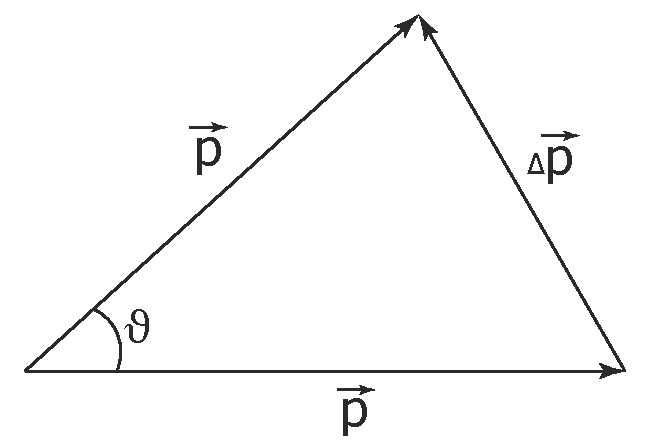
\includegraphics[width=.3\textwidth]{ppsin}
        \parbox{.3\textwidth}{\centering Треугольник импульсов}
    \end{tabular}
\end{table}

По формуле Резерфорда для угла рассеяния:
\[
    \ctg\frac{\theta}{2} = \frac{m_pv^2b}{ke^2Z} = \frac{2Tb}{ke^2Z}.
\]

Воспользовавшись известным тригонометрическим тождеством
\[
    \sin\frac{\theta}{2} = \frac{1}{\sqrt{1 + \ctg^2\frac{\theta}{2}}}
\]
и соотношениями \( p = \sqrt{2m_pT} \), \( m_pv^2 = 2T \), получим:
\[
    \Delta p = \frac{2p}{\sqrt{1 + \ctg^2\frac{\theta}{2}}} = \sqrt{\frac{4p^2}
    {1 + \left(\frac{m_pv^2b}{ke^2Z}\right)^2}} = \sqrt{\frac{8m_pT}{1 + \left(
    \frac{2Tb}{ke^2Z}\right)^2}}.
\]

\vspace*{2em}
\emph{Ответ:}
\vspace*{-1.7em}
\[
    \Delta p = \sqrt{\frac{8m_pT}{1 + \left(\frac{2Tb}{ke^2Z}\right)^2}}.
\]
\newpage
%-------------------------------------------------------------------------------
\emph{ИАЯФ 2.47.}
Вычислить для мезоатома водорода (в котором вместо электрона движется мезон,
имеющий тот же заряд, но массу в 207 раз больше):
\vspace*{-2em}
\begin{enumerate} \itemsep-.5em
    \item расстояние между мезоном и ядром в основном состоянии;
    \item длину волны резонансной линии;
    \item энергии связей основных состояний мезоатомов водорода, ядра которых
    протон и дейтрон.
\end{enumerate}

\vspace*{2em}
\emph{Решение:}
\begin{enumerate}
    \item По правилу квантования боровских орбит:
    \[
        L_n = \hbar n = mvr,
    \]
    где \( m = m_pm_\mu/(m_p + m_\mu) \) --- приведенная масса, \( m_p \) ---
    масса протона, \( m_\mu = 207m_e \) --- масса мезона. Отсюда \( v = \hbar n/(mr) \).
    
    Подставляем значение \( v \) во второй закон Ньютона
    \[
        m\frac{v^2}{r} = k\frac{e^2}{r^2}, \quad \frac{\hbar^2n^2}{mr} = ke^2.
    \]
    
    Найдем значение \( r \) в основном состоянии:
    \[
        r = \frac{\hbar^2 n^2}{mke^2} = \frac{\hbar^2}{m_\mu ke^2}\cdot\left(1 +
        \frac{m_\mu}{m_p}\right) = \frac{\hbar^2}{207m_eke^2}\cdot\left(1 +
        \frac{207m_e}{m_p}\right) = 2,\!85\cdot10^{-14}\text{ м}.
    \]
    
    \item Резонансная линия -- головная линия серии Лаймана:
    \[
        \omega = R_\mu\left(\frac{1}{1} - \frac{1}{4}\right) = \frac{3}{4}R_\mu.
    \]
    
    Постоянная Ридберга для мезоатома водорода:
    \[
        R_\mu = \frac{k^2e^4}{2\hbar^3}m = \frac{k^2e^4}{2\hbar^3}\cdot
        \frac{207m_em_p}{207m_e + m_p} = \frac{207m_p\cdot R}{207m_e + m_p}.
    \]
    
    Длина волны этой линии:
    \[
        \lambda = \frac{2\pi c}{\omega} = \frac{8\pi c}{3R_\mu} =
        \frac{8\pi c\cdot(207m_e + m_p)}{621m_p\cdot R} = 6,\!54\cdot10^{-11}
        \text{ м} = 654 \text{ пм}.        
    \]
    
    \item Энергия связи основного состояния мезоатома водорода, ядром которого
    является протон:
    \[
        E_\emph{п} = \hbar\omega_\infty = \hbar R_\mu\left(\frac{1}{1} - \frac{1}
        {\infty}\right) = \hbar R_\mu = \frac{207m_p\cdot\hbar R}{207m_e + m_p}
        = 2,\!53 \text{ КэВ}.
    \]
    Если ядром является дейтрон, то постоянная Ридберга:
    \[
        R_\emph{д} = \frac{k^2e^4}{2\hbar^3}\cdot\frac{207m_em_\emph{д}}{207m_e
        + m_\emph{д}} = \frac{207m_\emph{д}\cdot R}{207m_e + m_\emph{д}},
    \]
    где \( m_\emph{д} \) -- масса дейтрона.
    
    А энергия связи:
    \[
        E_\emph{д} = \hbar\omega_{\infty_\emph{д}} = \hbar R_\emph{д} =
        \frac{207m_\emph{д}\cdot\hbar R}{207m_e + m_\emph{д}}= 2,\!67
        \text{ КэВ}.
    \]
\end{enumerate}

\vspace*{2em}
\emph{Ответ:} а) \( r = 285 \)~фм; б) \( \lambda = 654 \)~пм;
в) \( E_\emph{п} = 2,\!53 \)~КэВ, \( E_\emph{д} = 2,\!67 \)~КэВ.
\newpage

%-------------------------------------------------------------------------------
\emph{ИАЯФ 3.32.}
Оценить минимально возможную энергию электронов в атоме He и
соответствующее расстояние электронов от ядра.

\vspace*{2em}
\emph{Решение:}

Полная энергия электрона в кулоновском поле для водородоподобного атома равна
\[
    E_1 = T + U = \frac{p^2}{2m_e} - \frac{Ze^2}{r} = \frac{p^2}{2m_e} -
    \frac{2e^2}{r}.
\]

Так как в атоме гелия два электрона, то энергия взаимодействия электронов с
атомом:
\[
    E_e = 2E_1 = 2\left(\frac{p^2}{2m_e} -
    \frac{2e^2}{r}\right) = \frac{p^2}{m_e} - \frac{4e^2}{r}.
\]

Также электроны будут взаимодействовать и между собой. Энергия их
взаимодействия, согласно закону Кулона:
\[
    E_\emph{в} = \frac{e^2}{d} = \frac{e^2}{2r}.
\]

Полная энергия электронов в атоме гелия будет равна сумме энергий:
\[
    E = E_e + E_\emph{в} = \frac{p^2}{m_e} - \frac{4e^2}{r} + \frac{e^2}{2r} =
    \frac{p^2}{m_e} - \frac{7e^2}{2r}.
\]

Из соотношения неопределенностей Гейзенберга, полагая \( \Delta r \sim r \),
\( \Delta p \sim p \):
\[
    r \cdot p \sim \hbar, \quad p \sim \frac{\hbar}{r}.
\]

Тогда энергия:
\[
    E = \frac{\hbar^2}{m_er^2} - \frac{7e^2}{2r}.
\]

Найдем минимум этой функции:
\[
    \der{E}{r} = -\frac{2\hbar^2}{mr^3} + \frac{7e^2}{2r^2} = 0,
\]
откуда расстояние электронов до ядра при минимальной энергии:
\[
    r = \frac{4\hbar^2}{7m_ee^2} = 3 \text{ пм}.
\]

Минимальное значение энергии:
\[
    E_{min} = \frac{\hbar^2}{m_e}\cdot\left(\frac{7e^2m_e}{4\hbar^2}\right)^2 -
    \frac{7e^2}{2}\cdot\frac{7e^2m_e}{4\hbar^2} = -\left(\frac{7}{4}\right)^2
    \frac{m_ee^4}{\hbar^2} = -83 \text{ эВ}.
\]

\vspace*{2em}
\emph{Ответ:}
\vspace*{-2.9em}
\[
    E_{min} = -\frac{49}{16}\frac{m_ee^4}{\hbar^2} = -83\text{ эВ},
    \  r = \frac{4\hbar^2}{7m_ee^2} = 3 \text{ пм}.
\]
\newpage

%-------------------------------------------------------------------------------
\emph{ИАЯФ 5.29.}
Выписать электронные конфигурации и с помощью правила Хунда найти основной
терм атомов: а) C и N; б) S и Cl. Электронные конфигурации этих атомов
соответствуют застройке электронных оболочек в нормальном порядке.

\vspace*{2em}
\emph{Решение:}
\begin{enumerate}
\item Электронная конфигурация атома \( ^6\)C: \( 1s^2 2s^2 2p^2 \).
    
    По правилам Хунда максимальное число \( S = 2 \cdot 1/2 = 1 \), наибольшее
    возможное \( L \) при таком \( S \), согласно принципу Паули, равно 1:
    \( ^3\mr{P} \).
    Так как подоболочка атома заполнена менее, чем наполовину, то число
    \( J = |L - S| = 0 \).
    
    Основной терм атома \( ^6 \)C: \( ^3\mr{P}_0 \).
    
    % ----- N
    Электронная конфигурация атома \( ^7\)N: \( 1s^2 2s^2 2p^3 \).

    По правилам Хунда максимальное число \( S = 3 \cdot 1/2 = 3/2 \), наибольшее
    возможное \( L \) при таком \( S \), согласно принципу Паули, равно 0. Так
    как подоболочка заполнена наполовину, то число \( J = L + S = 3/2 \).
    
    Основной терм атома \( ^7 \)N: \( ^4\mr{S}_{3/2} \).
    
    % ----- S
    \item Электронная конфигурация атома \( ^{16}\)S: \( 1s^2 2s^2 2p^6 3s^2
    3p^4 \).
    
    По правилам Хунда максимальное число \( S = (3 - 1) \cdot 1/2 = 1 \), наибольшее
    возможное \( L \) при таком \( S \), согласно принципу Паули, равно 1:
    \( ^3\mr{P} \).
    Так как подоболочка атома заполнена более, чем наполовину, то число
    \( J = L + S = 2 \).
    
    Основной терм атома \( ^{16} \)S: \( ^3\mr{P}_2 \).
    
    % ----- Cl
    Электронная конфигурация атома \( ^{17}\)Cl: \( 1s^2 2s^2 2p^6 3s^2
    3p^5 \).

    По правилам Хунда максимальное число \( S = (3 - 2) \cdot 1/2 = 1/2 \),
    наибольшее возможное \( L \) при таком \( S \), согласно принципу Паули,
    равно 1. Так как подоболочка заполнена более, чем наполовину, то число
    \( J = L + S = 3/2 \).
    
    Основной терм атома \( ^{17} \)Cl: \( ^2\mr{P}_{3/2} \).
\end{enumerate}

\vspace*{2em}
\emph{Ответ:} а) \( ^6 \)C: \( ^3\mr{P}_0 \), \( ^7 \)N: \( ^4\mr{S}_{3/2} \);
б) \( ^{16} \)S: \( ^3\mr{P}_2 \), \( ^{17} \)Cl: \( ^2\mr{P}_{3/2} \).
\newpage

%-------------------------------------------------------------------------------
\emph{ИОФ 5.192.}
При увеличении напряжения на рентгеновской трубке от \( U_1 = 10 \)~кВ до
\( U_2 = 20 \)~кВ интервал длин волн между \( K_\alpha \)-линией и коротковолновой
границей сплошного рентгеновского спектра увеличился в \( n = 3,0 \)~раза.
Определить порядковый номер элемента антикатода этой трубки, имея в виду, что
данный элемент является легким.

\vspace*{2em}
\emph{Решение:}

Длина волны коротковолновой границы сплошного рентгеновского спектра
определяется выражением
\[
    \lambda_\emph{кг} = \frac{2\pi c\hbar}{eU},
\]
где \( U \) -- напряжение на рентгеновской трубке.

Длина волны \( K_\alpha \)-линии:
\[
    \lambda_{K\alpha} = \frac{2\pi c}{\omega_{K\alpha}} = \frac{8\pi c}{3R(Z - 1)^2},
\]
где \( \omega_{K\alpha} = \frac{3}{4}R(Z - 1)^2 \) -- частота \( K_\alpha \)-линии.

Интервал между этими двумя линиями при увеличении напряжения увеличился в
\( n \) раз:
\vspace*{-1em}
\begin{align*}
    \lambda_{K\alpha} - \lambda_\emph{кг\,2} & = n(\lambda_{K\alpha} - 
    \lambda_\emph{кг\,1}); \\
    \frac{8\pi c}{3R(Z - 1)^2} - \frac{2\pi c\hbar}{eU_2} & = n\frac{8\pi c}
    {3R(Z - 1)^2} - n\frac{2\pi c\hbar}{eU_1}; \\
    \frac{4(n - 1)}{3R(Z - 1)^2} & = \frac{\hbar(nU_2 - U_1)}{eU_1U_2}; \\
    3R(Z - 1)^2 & = \frac{4eU_1U_2(n - 1)}{\hbar (nU_2 - U_1)}.
\end{align*}

Окончательно:
\[
    Z = 2\sqrt{\frac{eU_1(n - 1)}{3R\hbar\left(n - \frac{U_1}{U_2}\right)}} + 1 = 29.
\]

\vspace*{2em}
\emph{Ответ:}
\vspace*{-1.8em}
\[
    Z = 2\sqrt{\frac{eU_1(n - 1)}{3R\hbar\left(n - \frac{U_1}{U_2}\right)}} + 1 = 29.
\]
\end{document}
